\documentclass[crop,tikz]{standalone}



%\usepackage[dvipsnames]{xcolor}
\definecolor{col1}{HTML}{f3722c}
\definecolor{col2}{HTML}{f8961e}
\definecolor{col3}{HTML}{f9c74f}
\definecolor{col4}{HTML}{90be6d}
\definecolor{col5}{HTML}{43aa8b}
\definecolor{col6}{HTML}{577590}

\usepackage{pgfplots}
\pgfplotsset{compat=1.17}

\begin{document}

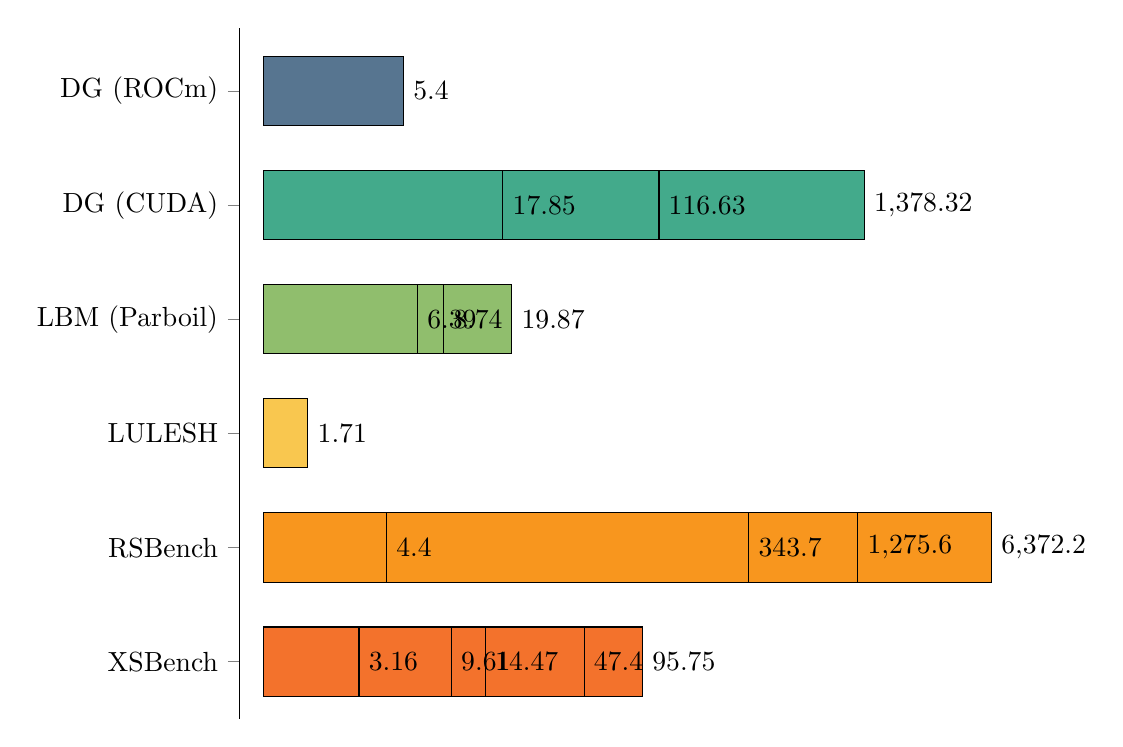
\begin{tikzpicture}
  \begin{axis}[
    xbar, xmin=0,
    ymin=0.5,
    xmode = log,
    point meta=rawx,
    width=12cm,
    bar width=25pt, % Set the y unit vector, that way, the plot will stretch to accommodate all bars
    % enlarge y limits={abs=1.5},
    % title={AD Overhead},
    hide x axis,
    % axis x line*=bottom,
    axis y line*=left,
    % ytick align=inside,
    %y interval=5pt,
    nodes near coords, nodes near coords align={horizontal},
    %symbolic y coords={XSBench},%, RSBench, LULESH, LBM (Parboil), DG (CUDA), DG (ROCm)},
    yticklabels={XSBench, RSBench, LULESH, LBM (Parboil), DG (CUDA), DG (ROCm)},
    ylabel style={name=ylabel},
    bar shift=0pt,
    ytick={1, 2, 3, 4, 5, 6}
  ]
  \addplot[fill=col1] coordinates{
    (3.16, 1) (9.61, 1) (14.47, 1) (47.40, 1) (95.75, 1)
  };
  
  \addplot[fill=col2] coordinates{
    (4.4, 2) (343.7, 2) (1275.6, 2) (6372.2, 2)
  };
  
  \addplot[fill=col3] coordinates{
    (1.71, 3)
    };

  \addplot[fill=col4] coordinates{
    (6.39, 4) (8.74, 4) (19.87, 4)
    };
    
  \addplot[fill=col5] coordinates{
    (17.85, 5) (116.63, 5) (1378.32, 5)
    };
    
  \addplot[fill=col6] coordinates{
    (5.4, 6)
    }; 
  \end{axis}
\end{tikzpicture}


%\begin{tikzpicture}
%    \begin{axis}[
%        xbar, xmin=0,
%        width=12cm,
%        height=3.5cm,
%        ylabel={Benchmark},
%        xlabel={AD Overhead},
%        symbolic y coords={XSBench, RSBench, LULESH, LBM (Parboil), DG (CUDA), DG (ROCm)},
%        nodes near coords, nodes near coords align={horizontal},
%        ytick=data,
%        bar width=17pt,
%        xtick=data,
%        nodes near coords,
%        nodes near coords align={vertical}
%    ]
%    % XSBench
%    \addplot coordinates{
%        (3.2, XSBench)
%        (4.4, RSBench)}
%    ;
%    
%    % RSBench
%    %\addplot coordinates{(4.4, RSBench)};
%    
%    % LULESH
%    %\addplot coordinates{(1.71, LULESH)};
%    
%    % LBM (Parboil)
%    %\addplot coordinates{(12.9, LBM (Parboil))};
%    
%    % DG (CUDA)
%    %\addplot coordinates{(27.5, DG (CUDA))};
%    
%    % DG (ROCm)
%    %\addplot coordinates{(5.4, DG (ROCm))};
%    
%    %\legend{XSBench, RSBench, LULESH, LBM (Parboil), DG (CUDA), DG (ROCm)}
%    \end{axis}
%\end{tikzpicture}
\end{document}